\documentclass{article}
\usepackage{amsmath,amssymb,fullpage,fancyhdr,graphicx}
\setlength{\parindent}{0in}
\title{AppStack Query Language}
\author{Gabe Fierro}
\date{}
\fancyhead{}
\renewcommand{\headrulewidth}{0.0pt}

\begin{document}
\maketitle
\section{Introduction} % (fold)
\label{sec:introduction}
The purpose of this query language is to facilitate the navigation of and collection of data within the functional graphs created by the user using the AppStack backend. This document has the goal of educating you, dear reader, on the structure of the graphs thus created and how one might use this query language.

\subsection{Graph Nodes} % (fold)
\label{sub:graph_nodes}

\begin{center}
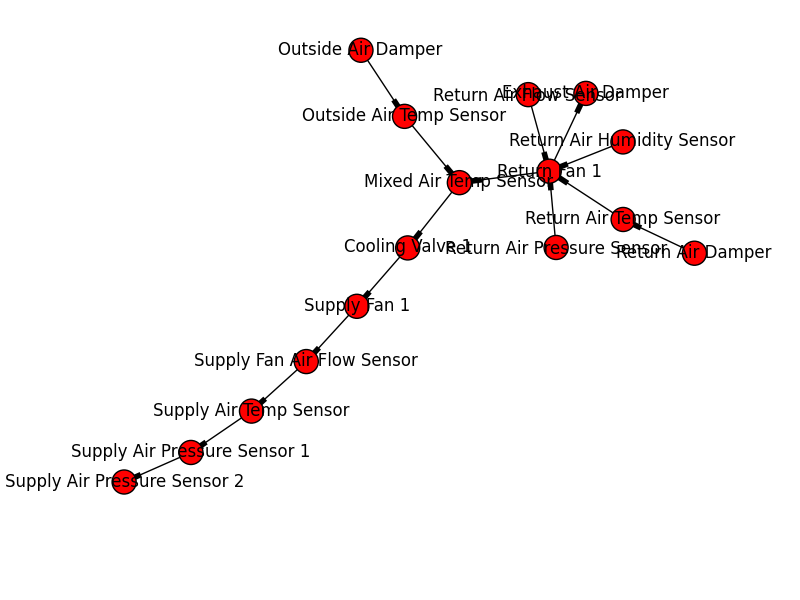
\includegraphics[scale=.8]{out.png}
\end{center}
Here is a sample functional graph of an Air Handler. A graph consists of a series of {\bf nodes} (representing physical objects in the system) connected by directed edges (representing the flow of the process from one node to another). As we can see in the graph above, the ``Outside Air Damper'' feeds into the ``Outside Air Temp Sensor'', which in turn feeds the ``Mixed Air Temp Sensor'', which is also fed by the ``Return Fan'', and so on. In this way we are able to capture the functional relationships between pieces in the system.
\\\\
Each {\bf node} is identified by three different attributes of differing degrees of uniqueness.
\begin{itemize}
	\item {\bf TYPE}: each object is identified by one of the 2-3 character types listed in \verb+node_types.type_dict+ (or listed by calling \verb+node_types.list_types()+). For example: ``AH'' $\rightarrow$ ``Air Handler'', ``DMP'' $\rightarrow$ ``Damper''.
	
	\item {\bf NAME}: each object is also initialized with a name, which is a string of arbitrary length, including ``[a-zA-Z]-:\_''. For example: ``Air Handler `'', ``Return Fan''
	
	\item {\bf TAG}: each object is usually tagged with some expected value when objects are initialized. For instance, an Air Handler Unit expects an outside air damper, which would be tagged as an ``OUT\_AIR\_DMP''. All tags are listed in \verb+node_types.list_tags()+ and can be translated with \verb+node_types.get_tag_name(tag)+.
	
	\item {\bf UID}: each object is additionally provisioned with a unique identification number, which is a UUID created upon initialization of the object. For example: ``c89bdbdd-e780-4f38-9523-9197d8161f6f''.
\end{itemize}
% subsection graph_nodes (end)

\subsection{Graphs Within Graphs} % (fold)
\label{sub:graphs_within_graphs}
Although this has not yet been integrated into the current sample code, the AppStack architecture supports (and indeed encourages) the encapsulation of smaller functional pieces (such as the figure above) within higher level objects which are themselves nodes in a larger graph.
\\\\
For example, the graph above \emph{functions} as an Air Handler, so it would be in another, larger, node that would be labelled as of the type ``AH''. This node would be part of a larger graph containing other nodes such as a ``cooling loop'' and ``hot water loop'' that would feed into the ``air handler'', represented by a directed edge.
% subsection graphs_within_graphs (end)

% section introduction (end)

\section{Query Language} % (fold)
\label{sec:query_language}
\subsection{What Can I Query?} % (fold)
\label{sub:what_can_i_query_}
Any valid query that you provide to the interpreter will return to you a set of nodes in the set of graphs that have been registered with the interpreter ( currently it is only the graph created in \verb+test.py+).
\\\\
You may query over any subset of the nodes that can be indicated by {\bf type}, {\bf name}, {\bf uid}, or {\bf relationship}.
% subsection what_can_i_query_ (end)

\subsection{Prefixes} % (fold)
\label{sub:prefixes}
In order to specify different objects in your queries, you use a small set of prefixes to help the interpreter distinguish.
\begin{center}
\begin{tabular}{| l | c | r |}
\hline
Prefix & What it Specifies & Examples of a {\bf Prefixed Expression}  \\ \hline
\#	&	Object Type/Class & \textbf{\#AH} (set of all Air Handlers), \textbf{\#DMP} (set of all Dampers) \\ \hline
\$ 	&	Object Name	& \textbf{\$Air Handler 1} (set of all air handlers named ``Air Handler '') \\ \hline
\%	&	Object UID & \textbf{\%ab61b939-a133-4d76-b9c4-a5d6fab7abf5} (the object with this UID) \\ \hline
\&  &	Object Tag & \textbf{\&OUT\_AIR\_DMP} (all objects tagged as an outside air damper) \\ \hline
@	&	Variable	& \textbf{@x} (returns the set previously stored in this variable) \\ \hline
\end{tabular}
\end{center}
% subsection prefixes (end)

\subsection{Query Format} % (fold)
\label{sub:query_format}
Queries take the basic form of:
\begin{center}
\verb+TARGET [DELIMITER SET [DELIMITER SET [...]]]+

\verb++

\begin{tabular}{| l | r |}
\hline
\verb+TARGET,SET+ & prefixed expression as indicated in the above table \\
& such as ``\#AH'', ``@varname'', ``\$Name of object'' \\ \hline
\verb+DELIMITER+& $>$: in the expression ``X $>$ Y'', X is ``upstream of'' \\
& or ``feeds into'' Y. \\
& $<$: in the expression ``X $<$ Y'', X is ``downstream of'' \\
& or ``is supplied by'' Y \\ \hline
\end{tabular}
\end{center}
The \verb+TARGET+ specifies the nature of the object(s) you'd like to receive upon resolving your query. \verb+TARGET+ and \verb+SET+ both take the form of either a {\bf prefixed expression}, which follows from the table above. \verb+DELIMITER+s specify the relationships between these sets.
% subsection query_format (end)
\subsection{Constructing a Query} % (fold)
\label{sub:constructing_a_query}
We construct a query from {\bf left} to {\bf right} by starting with our target set and appending a series of filters. Queries are perhaps most easily constructed by writing an English sentence describing the point(s) we are trying to find in the graph. For example:
\begin{center}\emph{``I want all sensors that measure the air from the return fan in this air handler''}\end{center}
We can immediately see that our {\bf target} are ``sensors'', so we begin the query by specifying that we want to return objects of \verb+TYPE+ ``sensor'', or ``\#SEN'':
\begin{center}\verb+#SEN+\end{center}
Now because we want sensors that measure air {\bf from} the return fan, this means that we want all sensors that are {\bf downstream} of the fan, so we use the ``$<$'' delimiter:
\begin{center}\verb+#SEN <+\end{center}
Lastly, we need to specify what exactly these sensors are downstream {\bf of}. We can specify the Return Fan by name (``\$Return Fan 1''):
\begin{center}\verb+#SEN < $Return Fan 1+\end{center}
However, the name ``Return Fan 1'' isn't guaranteed to be unique (other fans in other air handlers could be named ``Return Fan 1''), so we can use the UID of the object instead:
\begin{center}\verb+#SEN < %ab61b939-a133-4d76-b9c4-a5d6fab7abf5+\end{center}
which returns the correct list of sensors:
\begin{center}
	Mixed Air Temp Sensor d1786922-37e5-4bc9-8f4d-79c897c3d517
	
	Supply Fan Air Flow Sensor 146caeaa-482f-447a-8909-a30521ec56c2
	
	Supply Air Temp Sensor 49501c37-78c6-41fa-9659-f5aea37b9eb6
	
	Supply Air Pressure Sensor 1 7e171958-0eef-4c33-8373-a453ca63da55
	
	Supply Air Pressure Sensor 2 60c9cd79-e0ca-4710-a7a2-d1c428d946f6
\end{center}
Additionally, we can save the result of this query in a variable:
\begin{center}\verb+@sensors = #SEN < %ab61b939-a133-4d76-b9c4-a5d6fab7abf5+\end{center}
and then run further queries on that variable to search this new domain.

% subsection constructing_a_query (end)
\subsection{Additional Examples} % (fold)
\label{sub:additional_examples}

\begin{center}\emph{``I want all outside air dampers''}
	
	\verb+&OUT_AIR_DMP+
	
	Outside Air Damper 5b88969f-834e-4636-9686-c73afdabeb89
	
	Outside Air Damper 7f694301-2e04-44a9-b222-6c6ee0b26323
\end{center}

\begin{center}\emph{``I want all sensors in air handler 1 that are upstream of the cooling coil valve that feeds into the supply air fan''}
	
	\verb+(#SEN < $Air Handler 1) > &COO_VLV > &SUP_AIR_FAN+
	
	Mixed Air Temp Sensor 47c65480-bf3c-4343-af87-8c7820b2fd54
	
	Return Air Humidity Sensor 787c35e2-8961-46cc-b5db-2b304e390a5f
	
	Return Air Pressure Sensor f44d27ec-e698-4e87-9b70-d52e33869304
	
	Outside Air Temp Sensor 01ed9eba-1cd2-446b-97a5-b7dae7870714
	
	Return Air Flow Sensor 7c6bfdf7-5083-4667-83cb-1e5f1909e850

	Return Air Temp Sensor 540a778f-30bf-49c2-b06d-5c679621e3bc
\end{center}

\begin{center}\emph{``I want all cooling towers that feed the cooling valve that cools the air measured by the mixed air tmp sensor''}
	
	\verb+#TOW > ($Cooling Valve < $Mixed Air Temp Sensor)+
	
	Condensed Water Cooling Tower 96afc50a-ea13-4835-8e6d-b5cd289af2ad
\end{center}

% subsection additional_examples (end)
\subsection{Help} % (fold)
\label{sub:help}
Typing ``help'' into the interpreter gives you some additional commands you can use to help you learn what exactly you can query.
\\\\
You run the interpreter by running \verb+python lexerparser.py+ in the \verb+appstack+ directory.
% subsection help (end)
% section query_language (end)
\end{document}
